\documentclass[results.tex]{subfiles}
\begin{document}

\newpage

\subsection{Erdős–Rényi Graph}

For the Erdős–Rényi graph, the Graph Generator used the following parameters:

\begin{itemize}
\item Type of graph: Erdős–Rényi
\item Number of vertices: 20
\item Number of edges: 82
\item Probability: 82 / (20 * (20 - 1) / 2) = 0.43
\item Random generator seed: 1615826141222
\end{itemize}
and the model took the following parameters:
\begin{itemize}
\item Total defence quota each turn: 1.0
\item Probability with which the infection propagates: 1.0
\end{itemize}

\subsubsection{Deterministic Protection}

\subfile{ErdosRenyi/Deterministic/DeterministicTable.tex}

\newpage

\begin{figure}[!ht]
\centering
     \begin{subfigure}[b]{0.9\textwidth}
         \centering
         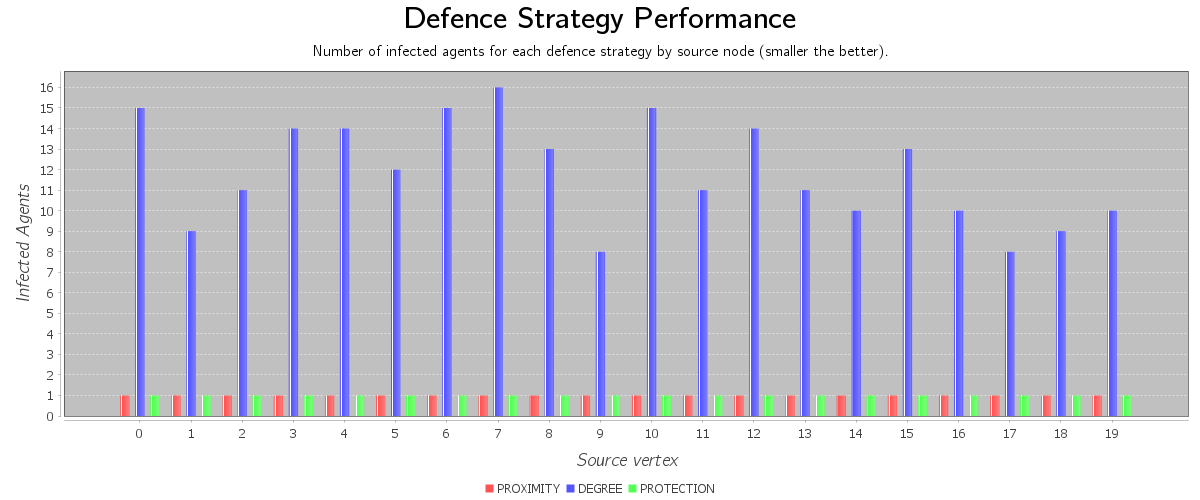
\includegraphics[width=\textwidth]{ErdosRenyi/Deterministic/DeterministicInfectedChart}
         %\caption{Infected}
         \label{fig:er-det-infected}
     \end{subfigure}
     \vfill
     \begin{subfigure}[b]{0.9\textwidth}
         \centering
         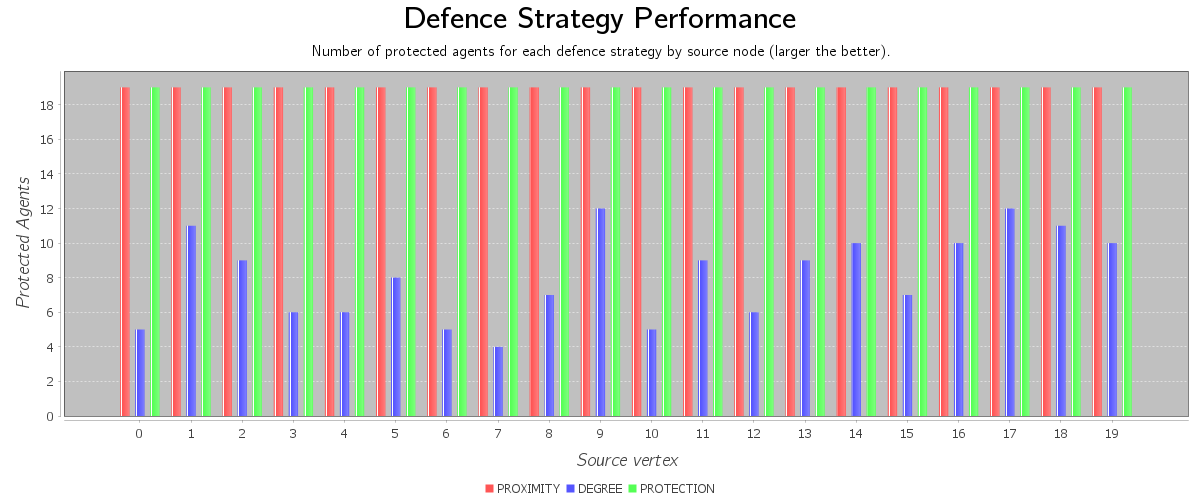
\includegraphics[width=\textwidth]{ErdosRenyi/Deterministic/DeterministicProtectedChart}
         %\caption{Protected}
         \label{fig:er-det-protected}
     \end{subfigure}
     \vfill
     \begin{subfigure}[b]{0.9\textwidth}
         \centering
         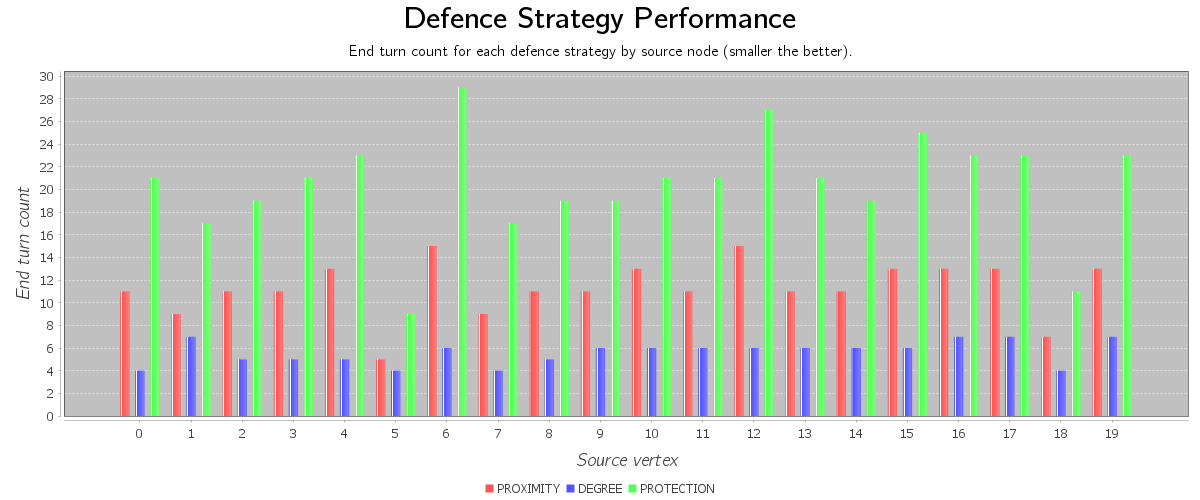
\includegraphics[width=\textwidth]{ErdosRenyi/Deterministic/DeterministicEndTurnChart}
         %\caption{End Turn}
         \label{fig:er-det-end}
     \end{subfigure}
        \caption{Model results on an Erdős–Rényi graph by source node for each defence strategy with deterministic initial protection allocation.}
        \label{fig:er-det-charts}
\end{figure}

\newpage


\subsubsection{Mixed Protection}

\subfile{ErdosRenyi/Mixed/MixedTable.tex}

\newpage

\begin{figure}[!ht]
\centering
     \begin{subfigure}[b]{0.9\textwidth}
         \centering
         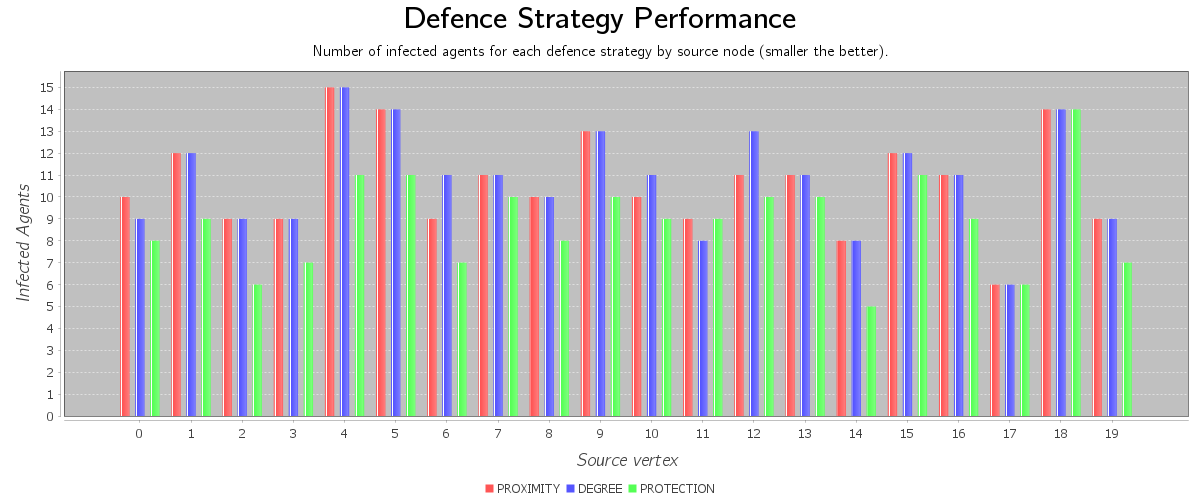
\includegraphics[width=\textwidth]{ErdosRenyi/Mixed/MixedInfectedChart}
         %\caption{Infected}
         \label{fig:er-mix-infected}
     \end{subfigure}
     \vfill
     \begin{subfigure}[b]{0.9\textwidth}
         \centering
         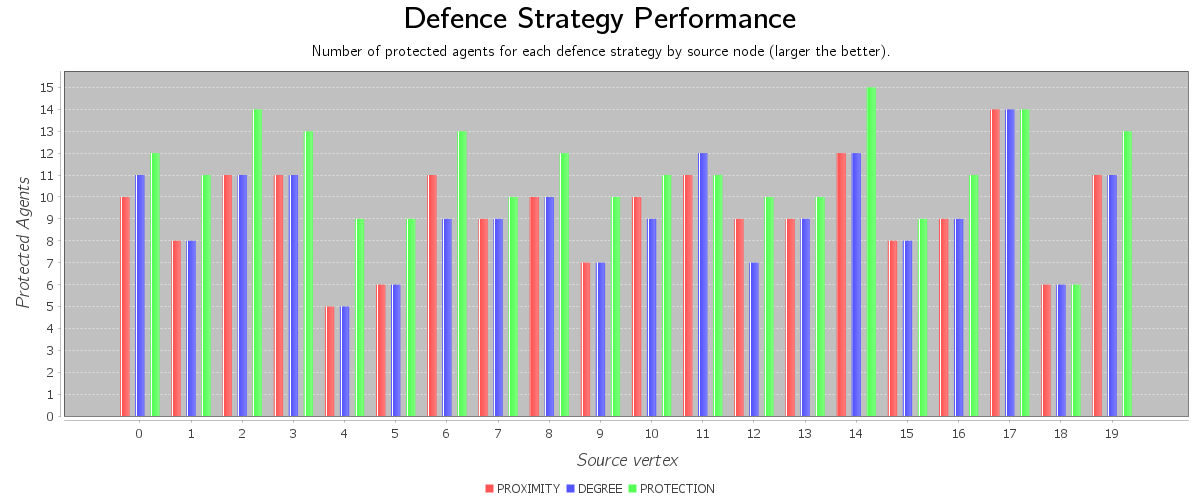
\includegraphics[width=\textwidth]{ErdosRenyi/Mixed/MixedProtectedChart}
         %\caption{Protected}
         \label{fig:er-mix-protected}
     \end{subfigure}
     \vfill
     \begin{subfigure}[b]{0.9\textwidth}
         \centering
         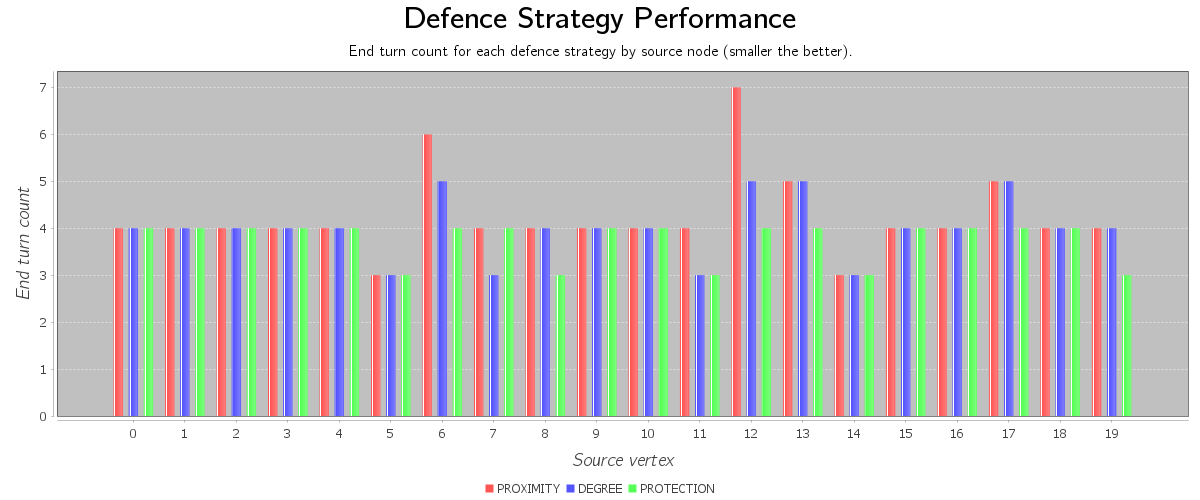
\includegraphics[width=\textwidth]{ErdosRenyi/Mixed/MixedEndTurnChart}
         %\caption{End Turn}
         \label{fig:er-mix-end}
     \end{subfigure}
        \caption{Model results on an Erdős–Rényi graph by source node for each defence strategy with mixed initial protection allocation.}
        \label{fig:er-mix-charts}
\end{figure}

\newpage 


\subsubsection{Random Protection}

\subfile{ErdosRenyi/Random/RandomTable.tex}

\newpage

\begin{figure}[!ht]
\centering
     \begin{subfigure}[b]{0.9\textwidth}
         \centering
         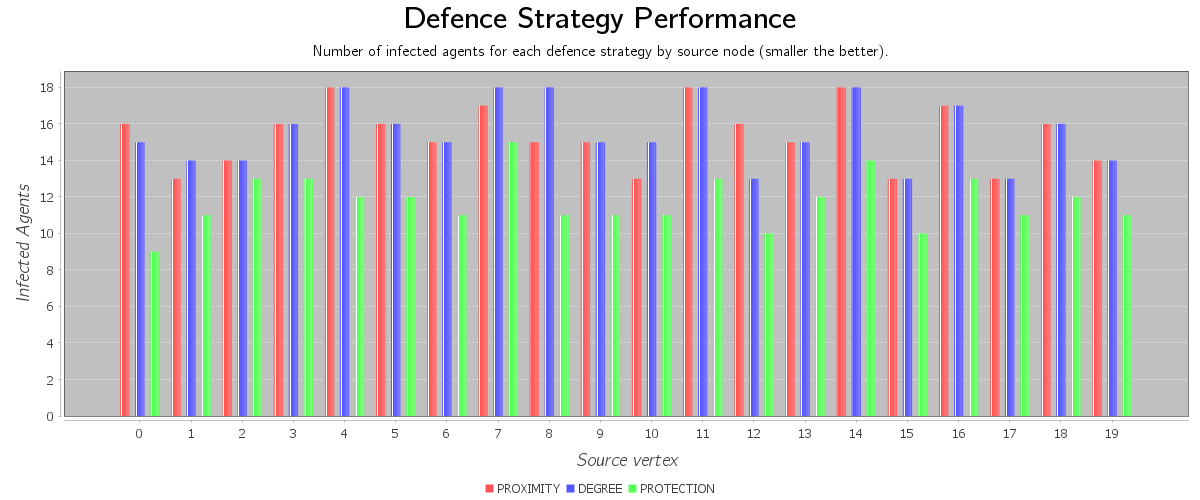
\includegraphics[width=\textwidth]{ErdosRenyi/Random/RandomInfectedChart}
         %\caption{Infected}
         \label{fig:er-ran-infected}
     \end{subfigure}
     \vfill
     \begin{subfigure}[b]{0.9\textwidth}
         \centering
         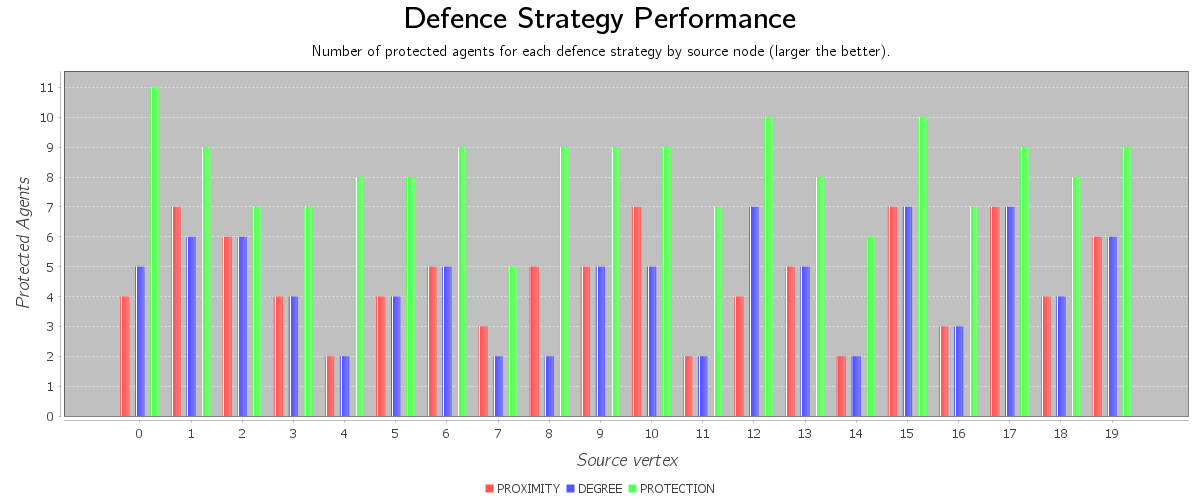
\includegraphics[width=\textwidth]{ErdosRenyi/Random/RandomProtectedChart}
         %\caption{Protected}
         \label{fig:er-ran-protected}
     \end{subfigure}
     \vfill
     \begin{subfigure}[b]{0.9\textwidth}
         \centering
         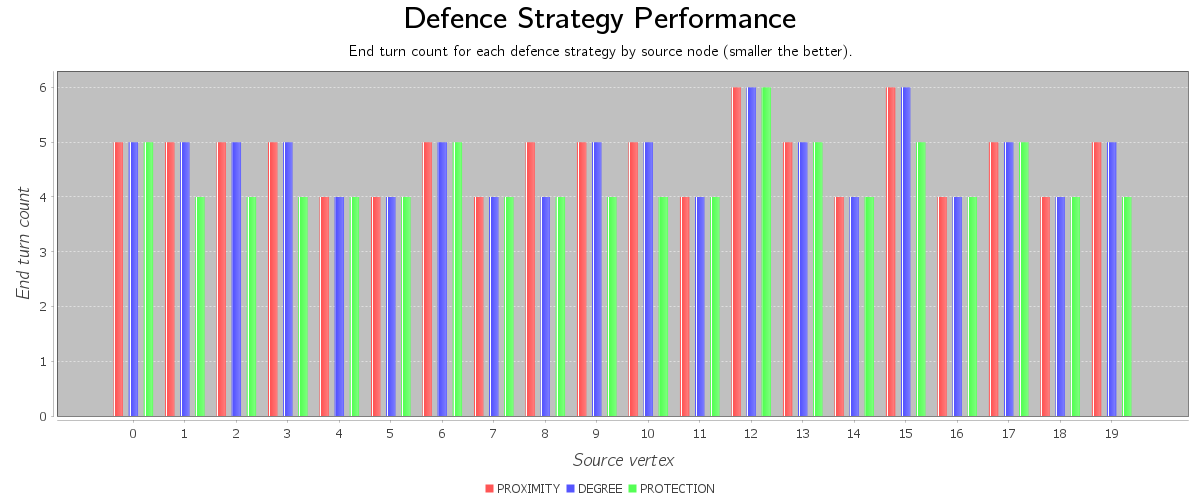
\includegraphics[width=\textwidth]{ErdosRenyi/Random/RandomEndTurnChart}
         %\caption{End Turn}
         \label{fig:er-ran-end}
     \end{subfigure}
        \caption{Model results on an Erdős–Rényi graph by source node for each defence strategy with random initial protection allocation.}
        \label{fig:er-ran-charts}
\end{figure}

\end{document}